\begin{frame}
\frametitle{Coding}
\begin{block}{Case study}
Analisi di un prototipo scritto in \textsc{Matlab} da Mark McCann, Paul Calamia
e Nir Ailon (Princeton University)
\end{block}

\begin{block}{}
\begin{itemize}
\item Analisi del codice
\item Creazione \emph{workflow}
\item Associazione tra \emph{workflow} del codice modello teorico
\item \textit{Debugging} e \textit{refactoring} del codice
\end{itemize}
\end{block}

\begin{block}{}
Parallelamente: \emph{code-reengineering}, in \emph{Python}
e \emph{OpenCV}
\end{block}
\end{frame}

\begin{frame}
\frametitle{\textsc{Matlab} code workflow}
\begin{figure}
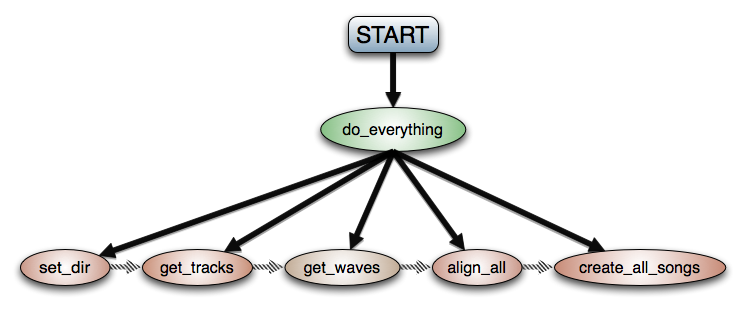
\includegraphics[width=\textwidth]{immagini/workflow.png}
\caption{\emph{Pipeline} codice \textsc{Matlab}}
\end{figure}
\end{frame}

